% % say that lammps and matlab were used in Introduction

\documentclass[BTech]{iitmdiss}
\usepackage{textcomp}
\usepackage{times}
%\usepackage{breqn}
\usepackage{tabularx}
\usepackage{url}
\usepackage{rotating}
\usepackage{adjustbox}
\usepackage{mathtools}
%\usepackage{geometry}
\usepackage{pbox}
\usepackage{multirow}
%\usepackage[paper=a4paper,left=1.5in,right=1in,top=1in,bottom=0.667in,nohead]{geometry}
\usepackage{float}
\usepackage{t1enc}
\newcommand{\angstrom}{\textup{\AA}}
\usepackage{wrapfig}
\usepackage{graphicx}
\usepackage{epstopdf}
\usepackage{lipsum}
\newcommand{\startsquarepar}{%
    \par\begingroup \parfillskip 0pt \relax}
\newcommand{\stopsquarepar}{%
    \par\endgroup}
\usepackage[driverfallback=dvipdfm]{hyperref} % hyperlinks for references.
\usepackage{amsmath} % easier math formulae, align, subequations \ldots
\ProvideTextCommand{\DJ}{OT1}{\raisebox{0.25ex}{-}\kern-0.4em D}
\usepackage{paracol}

\begin{document}

%%%%%%%%%%%%%%%%%%%%%%%%%%%%%%%%%%%%%%%%%%%%%%%%%%%%%%%%%%%%%%%%%%%%%%
% Title page
    \newcommand{\titleText}{Remote Center of Motion Constrained Planning for a 7DOF Robotic Arm}
    \newcommand{\authorText}{Suraj Rathi}
    \title{\titleText}

    \author{\authorText}

    \date{25 May 2023}
    \department{Mechanical Engineering}

%\nocite{*}
%\RequirePackage[ %compat2,a4paper,left=1.5in,right=1in,top=1in,bottom=0.667in,                nohead]{geometry}[2002/07/08]
    \newgeometry{left=1in,right=1.5in,top=1in,bottom=0.667in}
    \maketitle

%%%%%%%%%%%%%%%%%%%%%%%%%%%%%%%%%%%%%%%%%%%%%%%%%%%%%%%%%%%%%%%%%%%%%%
% Certificate
    \certificate

    \vspace*{0.5in}

    \noindent This is to certify that the thesis titled {\bf \titleText}, submitted by {\bf \authorText},
    to the Indian Institute of Technology, Madras, for
    the award of the degree of {\bf B.Tech}, is a bona fide
    record of the research work done by him under my supervision. The
    contents of this thesis, in full or in parts, have not been submitted
    to any other Institute or University for the award of any degree or
    diploma.

    \vspace*{1.5in}

    \begin{paracol}{2}
        \begin{singlespacing}
            \hspace*{-0.25in}
            \parbox{2.5in}{
                \noindent {\bf Dr.\ Nirav Patel} \\
                \noindent Research Guide \\
                \noindent \textit{Assistant Professor} \\
                \noindent Dept. of Engineering Design\\
                \noindent IIT-Madras, 600 036
            }
            \hspace*{1.56in}

            \vspace*{0.3in}
            \noindent Place: Chennai\\
            Date: 25$^{\textnormal{th}}$ May 2023

        \end{singlespacing}

        \switchcolumn
        \begin{singlespacing}
            \hspace*{-0.25in}
            \parbox{2.5in}{
                \noindent {\bf Dr.\ Sathyan Subbiah} \\
                \noindent Research Guide \\
                \noindent \textit{Professor} \\
                \noindent Dept. of Mechanical Engineering\\
                \noindent IIT-Madras, 600 036
            }
            \hspace*{1.56in}

            \vspace*{0.3in}
            \noindent Place: Chennai\\
            Date: 25$^{\textnormal{th}}$ May 2023

        \end{singlespacing}

    \end{paracol}


%%%%%%%%%%%%%%%%%%%%%%%%%%%%%%%%%%%%%%%%%%%%%%%%%%%%%%%%%%%%%%%%%%%%%%
% Acknowledgements
    \newgeometry{left=1.5in,right=1in,top=1in,bottom=0.667in}
    \acknowledgements

% TODO: Acknowledgementss
    \lipsum[1]


%%%%%%%%%%%%%%%%%%%%%%%%%%%%%%%%%%%%%%%%%%%%%%%%%%%%%%%%%%%%%%%%%%%%%%
% Abstract

    \abstract

% TODO: Abstract and Keywords
    \noindent KEYWORDS: \hspace*{0.5em} \parbox[t]{4.4in}{abc; ahds; hags.}

    \vspace*{24pt}
    \noindent
    In this project we attempt to build a realtime path planner satisfying a remote center of motion constraint.
    After ensuring the method will converge to a solution, the optimization objective is to minimize the total joint motion and to enforce motion limits on each joint.
    We set up a simulation using Open Robotics’ Gazebo to conduct our experiments in conjunction with the ROS platform.
    We worked to identify the challenges faced by planning in task space using Inverse-Kinematics.
    Sampling based methods were then used to improve the performance.
    Our work demonstrates the effectiveness of task space Inverse-Kinematics based methods.



    \pagebreak

    \disclaimer
    The Department of Mechanical Engineering, IIT Madras and the staff of IIT Madras, do not accept any responsibility for the truth, accuracy or completeness of material contained within or associated with this dissertation.

    Persons using all or any part of this material do so at their own risk, and not at the risk of the Department of Mechanical Engineering, IIT Madras and the staff of IIT Madras,

    This document, the associated hardware, software, drawings, and other material set out in the associated appendices should not be used for any other purpose: if they are so used, it is entirely at the risk of the user

    \pagebreak


%%%%%%%%%%%%%%%%%%%%%%%%%%%%%%%%%%%%%%%%%%%%%%%%%%%%%%%%%%%%%%%%%
% Table of contents etc.

    \begin{singlespace}
        \tableofcontents
        \thispagestyle{empty}

        \listoftables
        \addcontentsline{toc}{chapter}{LIST OF TABLES}
        \listoffigures
        \addcontentsline{toc}{chapter}{LIST OF FIGURES}
    \end{singlespace}


%%%%%%%%%%%%%%%%%%%%%%%%%%%%%%%%%%%%%%%%%%%%%%%%%%%%%%%%%%%%%%%%%%%%%%
% Abbreviations
% TODO: Abbreviations
    \newpage
    \begin{tabbing}

    \end{tabbing}
    \abbreviations

    \noindent
    \begin{tabbing}
        xxxxxxxxxxxxxx \= xxxxxxxxxxxxxxxxxxxxxxxxxxxxxxxxxxxxxxxxxxxxxxxx \kill
        \textbf{RCM} \> Remote Center of Motion\\
        \textbf{DOF} \> Degrees of Freedom\\

    \end{tabbing}

    \pagebreak

%%%%%%%%%%%%%%%%%%%%%%%%%%%%%%%%%%%%%%%%%%%%%%%%%%%%%%%%%%%%%%%%%%%%%%
% Notation
% TODO: Notations

    \chapter*{\centerline{NOTATIONS}}
    \addcontentsline{toc}{chapter}{NOTATIONS}

    \begin{singlespace}
        \begin{tabbing}
            xxxxxxxxxxx \= xxxxxxxxxxxxxxxxxxxxxxxxxxxxxxxxxxxxxxxxxxxxxxxx \kill
            $F$ \>  Force (N)\\
            $\delta$ \> Displacement (m)\\

        \end{tabbing}
    \end{singlespace}

    \pagebreak
    \clearpage

% The main text will follow from this point so set the page numbering
% to arabic from here on.
    \pagenumbering{arabic}


%%%%%%%%%%%%%%%%%%%%%%%%%%%%%%%%%%%%%%%%%%%%%%%%%%
% Introduction.


    \chapter{INTRODUCTION}\label{ch:intro}


    \section{Motivation}\label{sec:motiv}
    Laparoscopic surgery, commonly know as `keyhole' surgery, is a procedure where a surgeon accesses the inside of
    the abdomen and pelvis without having to make a large incision.
    We are attempting to use a LBR iiwa 7~\cite{AG} arm produced by KUKA, which is a 7DOF robotic arm, to perform such a surgery.  % TODO: Add a reference?

    In this surgery, a small incision is made on the skin, and the surgical instruments are manipulated through that incision.
    We have model this as a cylindrical, and later circular, shape.
    The endeffector must always enter through the upper circular face and exit through the lower circular face.
    It must always pass through some volume of the cylinder and cannot intersect with the curved surface.
    An illustration can be seen in~\ref{fig:RCM}.
    This is quite similar to the `Remote Center of Motion' (RCM) constraint and henceforth, when we use the term RCM we will be referring to the aforementioned constraint.

    \begin{figure}
        \centering
        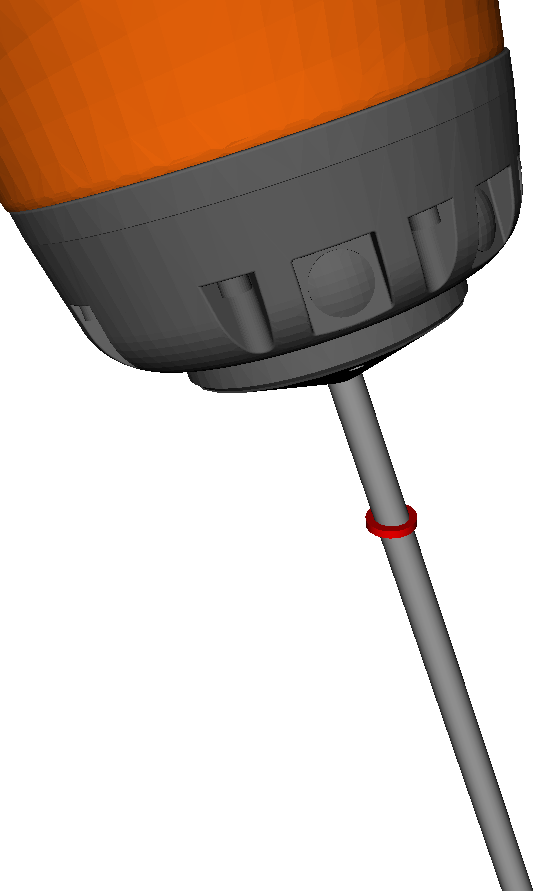
\includegraphics[height= 0.5\textwidth]{./img/rcm-constraint}
        \caption{A depiction of the Laproscopic surgery constraint as implemented in our work. The orange and gray objects are part of the robotic arm and the red cylinder represents the volume through which the end-effector must always pass.}
        \label{fig:RCM}
    \end{figure}

    We wished to implement a real-time path planner that can satisfy the RCM constraint.


    \section{Survey of Existing Methods}

    \subsection{Path Planners}
    Our survey of existing planning methods was primarily done by surveying the available algorithms in ROS MoveIT \cite{Coleman_Sucan_Chitta_Correll_2014}.
    This library provides a unified frontend to various motion planners and integrates wil the FCL collision checker, and with simulation and visualization software through the ROS framework.
    We must note that these planners are optimized for a general purpose use case.
    Our robot is very simple, and when it is inside the RCM, we observed that the links do not collide with each-other we do not require all the complexities and features of these full scale planners.

    % TODO: go into detail about different planners?

    A second technique can be used, wherein if we can generate a path in task space (i.e. in the coordinates of the tip of the end-effector),
    we can use Inverse Kinematics (IK) to generate the required joint angles in configuration space. This approach generally has the following problems.
    \begin{enumerate}
        \item Solving the IK problem may be slow
        \item There may be no IK solution for a given pose
        \item The IK solution will not be unique
        \item There may be large jumps in IK solutions between two consecutive points in the path.
    \end{enumerate}

    The Kinematics and Dynamics Library (KDL)~\cite{kdl-url} is default solver used by MoveIT for solving forward and inverse kinematics problems.
    We can also use the IKFast algorithm to generate analytical solutions for a given robot configuration.

    \subsection{7DOF Robot Control}

    Another challenge with working with this robot is its the over-actuated nature.
    To control the six DOF of the end-effector pose, we need to specify the joint angle of seven actuators.
    This leaves us with one extra DOF.
    In literature, we have seen others use that DOF to implement better obstacle avoidance~\cite{Doliwa_2020} and lock a single joint to get closed form kinematics~\cite{Asthana}


    \section{Objectives}


    \chapter{METHODOLGY}\label{ch:introm}


%%%%%%%%%%%%%%%%%%%%%%%%%%%%%%%%%%%%%%%%%%%%%%%%%%%%%%%%%%%%
% Appendices.

    \appendix


    \chapter{MATLAB code for polymer network creation} \label{code}

    Just put in text as you would into any chapter with sections and whatnot. Thats the end of it.

%%%%%%%%%%%%%%%%%%%%%%%%%%%%%%%%%%%%%%%%%%%%%%%%%%%%%%%%%%%%
% Bibliography.

    \begin{singlespace}
        \bibliography{thesis_template}
        % \bibliographystyle{iitm}
    \end{singlespace}

\end{document}
